\documentclass[1p]{elsarticle_modified}
%\bibliographystyle{elsarticle-num}

%\usepackage[colorlinks]{hyperref}
%\usepackage{abbrmath_seonhwa} %\Abb, \Ascr, \Acal ,\Abf, \Afrak
\usepackage{amsfonts}
\usepackage{amssymb}
\usepackage{amsmath}
\usepackage{amsthm}
\usepackage{scalefnt}
\usepackage{amsbsy}
\usepackage{kotex}
\usepackage{caption}
\usepackage{subfig}
\usepackage{color}
\usepackage{graphicx}
\usepackage{xcolor} %% white, black, red, green, blue, cyan, magenta, yellow
\usepackage{float}
\usepackage{setspace}
\usepackage{hyperref}

\usepackage{tikz}
\usetikzlibrary{arrows}

\usepackage{multirow}
\usepackage{array} % fixed length table
\usepackage{hhline}

%%%%%%%%%%%%%%%%%%%%%
\makeatletter
\renewcommand*\env@matrix[1][\arraystretch]{%
	\edef\arraystretch{#1}%
	\hskip -\arraycolsep
	\let\@ifnextchar\new@ifnextchar
	\array{*\c@MaxMatrixCols c}}
\makeatother %https://tex.stackexchange.com/questions/14071/how-can-i-increase-the-line-spacing-in-a-matrix
%%%%%%%%%%%%%%%

\usepackage[normalem]{ulem}

\newcommand{\msout}[1]{\ifmmode\text{\sout{\ensuremath{#1}}}\else\sout{#1}\fi}
%SOURCE: \msout is \stkout macro in https://tex.stackexchange.com/questions/20609/strikeout-in-math-mode

\newcommand{\cancel}[1]{
	\ifmmode
	{\color{red}\msout{#1}}
	\else
	{\color{red}\sout{#1}}
	\fi
}

\newcommand{\add}[1]{
	{\color{blue}\uwave{#1}}
}

\newcommand{\replace}[2]{
	\ifmmode
	{\color{red}\msout{#1}}{\color{blue}\uwave{#2}}
	\else
	{\color{red}\sout{#1}}{\color{blue}\uwave{#2}}
	\fi
}

\newcommand{\Sol}{\mathcal{S}} %segment
\newcommand{\D}{D} %diagram
\newcommand{\A}{\mathcal{A}} %arc


%%%%%%%%%%%%%%%%%%%%%%%%%%%%%5 test

\def\sl{\operatorname{\textup{SL}}(2,\Cbb)}
\def\psl{\operatorname{\textup{PSL}}(2,\Cbb)}
\def\quan{\mkern 1mu \triangleright \mkern 1mu}

\theoremstyle{definition}
\newtheorem{thm}{Theorem}[section]
\newtheorem{prop}[thm]{Proposition}
\newtheorem{lem}[thm]{Lemma}
\newtheorem{ques}[thm]{Question}
\newtheorem{cor}[thm]{Corollary}
\newtheorem{defn}[thm]{Definition}
\newtheorem{exam}[thm]{Example}
\newtheorem{rmk}[thm]{Remark}
\newtheorem{alg}[thm]{Algorithm}

\newcommand{\I}{\sqrt{-1}}
\begin{document}

%\begin{frontmatter}
%
%\title{Boundary parabolic representations of knots up to 8 crossings}
%
%%% Group authors per affiliation:
%\author{Yunhi Cho} 
%\address{Department of Mathematics, University of Seoul, Seoul, Korea}
%\ead{yhcho@uos.ac.kr}
%
%
%\author{Seonhwa Kim} %\fnref{s_kim}}
%\address{Center for Geometry and Physics, Institute for Basic Science, Pohang, 37673, Korea}
%\ead{ryeona17@ibs.re.kr}
%
%\author{Hyuk Kim}
%\address{Department of Mathematical Sciences, Seoul National University, Seoul 08826, Korea}
%\ead{hyukkim@snu.ac.kr}
%
%\author{Seokbeom Yoon}
%\address{Department of Mathematical Sciences, Seoul National University, Seoul, 08826,  Korea}
%\ead{sbyoon15@snu.ac.kr}
%
%\begin{abstract}
%We find all boundary parabolic representation of knots up to 8 crossings.
%
%\end{abstract}
%\begin{keyword}
%    \MSC[2010] 57M25 
%\end{keyword}
%
%\end{frontmatter}

%\linenumbers
%\tableofcontents
%
\newcommand\colored[1]{\textcolor{white}{\rule[-0.35ex]{0.8em}{1.4ex}}\kern-0.8em\color{red} #1}%
%\newcommand\colored[1]{\textcolor{white}{ #1}\kern-2.17ex	\textcolor{white}{ #1}\kern-1.81ex	\textcolor{white}{ #1}\kern-2.15ex\color{red}#1	}

{\Large $\underline{12n_{0792}~(K12n_{0792})}$}

\setlength{\tabcolsep}{10pt}
\renewcommand{\arraystretch}{1.6}
\vspace{1cm}\begin{tabular}{m{100pt}>{\centering\arraybackslash}m{274pt}}
\multirow{5}{120pt}{
	\centering
	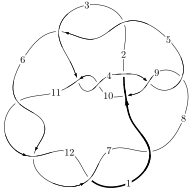
\includegraphics[width=112pt]{../../../GIT/diagram.site/Diagrams/png/2881_12n_0792.png}\\
\ \ \ A knot diagram\footnotemark}&
\allowdisplaybreaks
\textbf{Linearized knot diagam} \\
\cline{2-2}
 &
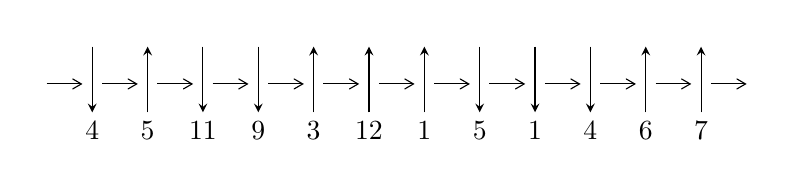
\begin{tikzpicture}[x=20pt, y=17pt]
	% nodes
	\node (C0) at (0, 0) {};
	\node (C1) at (1, 0) {};
	\node (C1U) at (1, +1) {};
	\node (C1D) at (1, -1) {4};

	\node (C2) at (2, 0) {};
	\node (C2U) at (2, +1) {};
	\node (C2D) at (2, -1) {5};

	\node (C3) at (3, 0) {};
	\node (C3U) at (3, +1) {};
	\node (C3D) at (3, -1) {11};

	\node (C4) at (4, 0) {};
	\node (C4U) at (4, +1) {};
	\node (C4D) at (4, -1) {9};

	\node (C5) at (5, 0) {};
	\node (C5U) at (5, +1) {};
	\node (C5D) at (5, -1) {3};

	\node (C6) at (6, 0) {};
	\node (C6U) at (6, +1) {};
	\node (C6D) at (6, -1) {12};

	\node (C7) at (7, 0) {};
	\node (C7U) at (7, +1) {};
	\node (C7D) at (7, -1) {1};

	\node (C8) at (8, 0) {};
	\node (C8U) at (8, +1) {};
	\node (C8D) at (8, -1) {5};

	\node (C9) at (9, 0) {};
	\node (C9U) at (9, +1) {};
	\node (C9D) at (9, -1) {1};

	\node (C10) at (10, 0) {};
	\node (C10U) at (10, +1) {};
	\node (C10D) at (10, -1) {4};

	\node (C11) at (11, 0) {};
	\node (C11U) at (11, +1) {};
	\node (C11D) at (11, -1) {6};

	\node (C12) at (12, 0) {};
	\node (C12U) at (12, +1) {};
	\node (C12D) at (12, -1) {7};
	\node (C13) at (13, 0) {};

	% arrows
	\draw[->,>={angle 60}]
	(C0) edge (C1) (C1) edge (C2) (C2) edge (C3) (C3) edge (C4) (C4) edge (C5) (C5) edge (C6) (C6) edge (C7) (C7) edge (C8) (C8) edge (C9) (C9) edge (C10) (C10) edge (C11) (C11) edge (C12) (C12) edge (C13) ;	\draw[->,>=stealth]
	(C1U) edge (C1D) (C2D) edge (C2U) (C3U) edge (C3D) (C4U) edge (C4D) (C5D) edge (C5U) (C6D) edge (C6U) (C7D) edge (C7U) (C8U) edge (C8D) (C9U) edge (C9D) (C10U) edge (C10D) (C11D) edge (C11U) (C12D) edge (C12U) ;
	\end{tikzpicture} \\
\hhline{~~} \\& 
\textbf{Solving Sequence} \\ \cline{2-2} 
 &
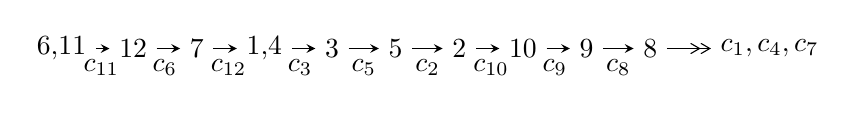
\begin{tikzpicture}[x=23pt, y=7pt]
	% node
	\node (A0) at (-1/8, 0) {6,11};
	\node (A1) at (1, 0) {12};
	\node (A2) at (2, 0) {7};
	\node (A3) at (49/16, 0) {1,4};
	\node (A4) at (33/8, 0) {3};
	\node (A5) at (41/8, 0) {5};
	\node (A6) at (49/8, 0) {2};
	\node (A7) at (57/8, 0) {10};
	\node (A8) at (65/8, 0) {9};
	\node (A9) at (73/8, 0) {8};
	\node (C1) at (1/2, -1) {$c_{11}$};
	\node (C2) at (3/2, -1) {$c_{6}$};
	\node (C3) at (5/2, -1) {$c_{12}$};
	\node (C4) at (29/8, -1) {$c_{3}$};
	\node (C5) at (37/8, -1) {$c_{5}$};
	\node (C6) at (45/8, -1) {$c_{2}$};
	\node (C7) at (53/8, -1) {$c_{10}$};
	\node (C8) at (61/8, -1) {$c_{9}$};
	\node (C9) at (69/8, -1) {$c_{8}$};
	\node (A10) at (11, 0) {$c_{1},c_{4},c_{7}$};

	% edge
	\draw[->,>=stealth]	
	(A0) edge (A1) (A1) edge (A2) (A2) edge (A3) (A3) edge (A4) (A4) edge (A5) (A5) edge (A6) (A6) edge (A7) (A7) edge (A8) (A8) edge (A9) ;
	\draw[->>,>={angle 60}]	
	(A9) edge (A10);
\end{tikzpicture} \\ 

\end{tabular} \\

\footnotetext{
The image of knot diagram is generated by the software ``\textbf{Draw programme}" developed by Andrew Bartholomew(\url{http://www.layer8.co.uk/maths/draw/index.htm\#Running-draw}), where we modified some parts for our purpose(\url{https://github.com/CATsTAILs/LinksPainter}).
}\phantom \\ \newline 
\centering \textbf{Ideals for irreducible components\footnotemark of $X_{\text{par}}$} 
 
\begin{align*}
I^u_{1}&=\langle 
3.07628\times10^{46} u^{52}-1.00351\times10^{47} u^{51}+\cdots+3.48741\times10^{47} b+1.73101\times10^{48},\\
\phantom{I^u_{1}}&\phantom{= \langle  }-1.34583\times10^{48} u^{52}+5.85153\times10^{47} u^{51}+\cdots+6.62608\times10^{48} a-2.02004\times10^{48},\;u^{53}+u^{52}+\cdots+2 u+19\rangle \\
I^u_{2}&=\langle 
u^{10}-7 u^8+u^7+17 u^6-5 u^5-16 u^4+7 u^3+4 u^2+b-2 u,\\
\phantom{I^u_{2}}&\phantom{= \langle  }- u^{10}+7 u^8- u^7-17 u^6+5 u^5+16 u^4-7 u^3-5 u^2+a+2 u+2,\\
\phantom{I^u_{2}}&\phantom{= \langle  }u^{14}-10 u^{12}+u^{11}+39 u^{10}-8 u^9-74 u^8+23 u^7+69 u^6-28 u^5-28 u^4+13 u^3+4 u^2-2 u+1\rangle \\
\\
\end{align*}
\raggedright * 2 irreducible components of $\dim_{\mathbb{C}}=0$, with total 67 representations.\\
\footnotetext{All coefficients of polynomials are rational numbers. But the coefficients are sometimes approximated in decimal forms when there is not enough margin.}
\newpage
\renewcommand{\arraystretch}{1}
\centering \section*{I. $I^u_{1}= \langle 3.08\times10^{46} u^{52}-1.00\times10^{47} u^{51}+\cdots+3.49\times10^{47} b+1.73\times10^{48},\;-1.35\times10^{48} u^{52}+5.85\times10^{47} u^{51}+\cdots+6.63\times10^{48} a-2.02\times10^{48},\;u^{53}+u^{52}+\cdots+2 u+19 \rangle$}
\flushleft \textbf{(i) Arc colorings}\\
\begin{tabular}{m{7pt} m{180pt} m{7pt} m{180pt} }
\flushright $a_{6}=$&$\begin{pmatrix}0\\u\end{pmatrix}$ \\
\flushright $a_{11}=$&$\begin{pmatrix}1\\0\end{pmatrix}$ \\
\flushright $a_{12}=$&$\begin{pmatrix}1\\- u^2\end{pmatrix}$ \\
\flushright $a_{7}=$&$\begin{pmatrix}u\\- u^3+u\end{pmatrix}$ \\
\flushright $a_{1}=$&$\begin{pmatrix}- u^2+1\\u^4-2 u^2\end{pmatrix}$ \\
\flushright $a_{4}=$&$\begin{pmatrix}0.203111 u^{52}-0.0883105 u^{51}+\cdots-9.46298 u+0.304862\\-0.0882110 u^{52}+0.287753 u^{51}+\cdots-1.72583 u-4.96359\end{pmatrix}$ \\
\flushright $a_{3}=$&$\begin{pmatrix}0.114900 u^{52}+0.199442 u^{51}+\cdots-11.1888 u-4.65873\\-0.0882110 u^{52}+0.287753 u^{51}+\cdots-1.72583 u-4.96359\end{pmatrix}$ \\
\flushright $a_{5}=$&$\begin{pmatrix}0.0908917 u^{52}+0.0768978 u^{51}+\cdots-7.10988 u-3.08929\\0.0260187 u^{52}+0.0838960 u^{51}+\cdots-5.33771 u-3.10420\end{pmatrix}$ \\
\flushright $a_{2}=$&$\begin{pmatrix}0.0279811 u^{52}+0.0401943 u^{51}+\cdots+3.61598 u+4.82383\\-0.0143374 u^{52}-0.198875 u^{51}+\cdots+4.54528 u+3.00459\end{pmatrix}$ \\
\flushright $a_{10}=$&$\begin{pmatrix}-0.109349 u^{52}+0.187204 u^{51}+\cdots-5.22764 u-4.01238\\0.272728 u^{52}+0.00219298 u^{51}+\cdots-4.61603 u-0.998578\end{pmatrix}$ \\
\flushright $a_{9}=$&$\begin{pmatrix}0.0602843 u^{52}+0.218936 u^{51}+\cdots-9.13144 u-3.51075\\0.120808 u^{52}-0.0288635 u^{51}+\cdots-1.02731 u-0.112491\end{pmatrix}$ \\
\flushright $a_{8}=$&$\begin{pmatrix}u^3-2 u\\- u^5+3 u^3- u\end{pmatrix}$\\&\end{tabular}
\flushleft \textbf{(ii) Obstruction class $= -1$}\\~\\
\flushleft \textbf{(iii) Cusp Shapes $= 0.0556426 u^{52}+0.289899 u^{51}+\cdots+16.8530 u+6.93721$}\\~\\
\newpage\renewcommand{\arraystretch}{1}
\flushleft \textbf{(iv) u-Polynomials at the component}\newline \\
\begin{tabular}{m{50pt}|m{274pt}}
Crossings & \hspace{64pt}u-Polynomials at each crossing \\
\hline $$\begin{aligned}c_{1}\end{aligned}$$&$\begin{aligned}
&u^{53}-8 u^{52}+\cdots-25 u+1
\end{aligned}$\\
\hline $$\begin{aligned}c_{2},c_{5}\end{aligned}$$&$\begin{aligned}
&u^{53}-18 u^{51}+\cdots- u+683
\end{aligned}$\\
\hline $$\begin{aligned}c_{3},c_{10}\end{aligned}$$&$\begin{aligned}
&u^{53}- u^{52}+\cdots+996 u-745
\end{aligned}$\\
\hline $$\begin{aligned}c_{4},c_{8}\end{aligned}$$&$\begin{aligned}
&u^{53}+2 u^{52}+\cdots-13 u-1
\end{aligned}$\\
\hline $$\begin{aligned}c_{6},c_{7},c_{11}\\c_{12}\end{aligned}$$&$\begin{aligned}
&u^{53}- u^{52}+\cdots+2 u-19
\end{aligned}$\\
\hline $$\begin{aligned}c_{9}\end{aligned}$$&$\begin{aligned}
&u^{53}+3 u^{52}+\cdots+26 u-1
\end{aligned}$\\
\hline
\end{tabular}\\~\\
\newpage\renewcommand{\arraystretch}{1}
\flushleft \textbf{(v) Riley Polynomials at the component}\newline \\
\begin{tabular}{m{50pt}|m{274pt}}
Crossings & \hspace{64pt}Riley Polynomials at each crossing \\
\hline $$\begin{aligned}c_{1}\end{aligned}$$&$\begin{aligned}
&y^{53}-36 y^{52}+\cdots+47 y-1
\end{aligned}$\\
\hline $$\begin{aligned}c_{2},c_{5}\end{aligned}$$&$\begin{aligned}
&y^{53}-36 y^{52}+\cdots+10124793 y-466489
\end{aligned}$\\
\hline $$\begin{aligned}c_{3},c_{10}\end{aligned}$$&$\begin{aligned}
&y^{53}+31 y^{52}+\cdots-10501844 y-555025
\end{aligned}$\\
\hline $$\begin{aligned}c_{4},c_{8}\end{aligned}$$&$\begin{aligned}
&y^{53}+22 y^{52}+\cdots+167 y-1
\end{aligned}$\\
\hline $$\begin{aligned}c_{6},c_{7},c_{11}\\c_{12}\end{aligned}$$&$\begin{aligned}
&y^{53}-65 y^{52}+\cdots+5324 y-361
\end{aligned}$\\
\hline $$\begin{aligned}c_{9}\end{aligned}$$&$\begin{aligned}
&y^{53}-33 y^{52}+\cdots+392 y-1
\end{aligned}$\\
\hline
\end{tabular}\\~\\
\newpage\flushleft \textbf{(vi) Complex Volumes and Cusp Shapes}
$$\begin{array}{c|c|c}  
\text{Solutions to }I^u_{1}& \I (\text{vol} + \sqrt{-1}CS) & \text{Cusp shape}\\
 \hline 
\begin{aligned}
u &= \phantom{-}0.976765 + 0.204315 I \\
a &= -0.695066 - 1.196400 I \\
b &= -0.341850 + 0.765716 I\end{aligned}
 & \phantom{-}3.70234 + 2.85475 I & \phantom{-}7.56242 - 7.71874 I \\ \hline\begin{aligned}
u &= \phantom{-}0.976765 - 0.204315 I \\
a &= -0.695066 + 1.196400 I \\
b &= -0.341850 - 0.765716 I\end{aligned}
 & \phantom{-}3.70234 - 2.85475 I & \phantom{-}7.56242 + 7.71874 I \\ \hline\begin{aligned}
u &= \phantom{-}0.830103 + 0.663239 I \\
a &= \phantom{-}0.622792 + 0.940843 I \\
b &= \phantom{-}0.68077 - 1.27126 I\end{aligned}
 & \phantom{-}1.17909 + 10.63840 I & \phantom{-}4.37034 - 8.18411 I \\ \hline\begin{aligned}
u &= \phantom{-}0.830103 - 0.663239 I \\
a &= \phantom{-}0.622792 - 0.940843 I \\
b &= \phantom{-}0.68077 + 1.27126 I\end{aligned}
 & \phantom{-}1.17909 - 10.63840 I & \phantom{-}4.37034 + 8.18411 I \\ \hline\begin{aligned}
u &= -0.672364 + 0.631114 I \\
a &= \phantom{-}0.755869 - 0.889133 I \\
b &= \phantom{-}0.567716 + 1.241920 I\end{aligned}
 & -0.25800 - 4.19233 I & \phantom{-}2.11175 + 4.57513 I \\ \hline\begin{aligned}
u &= -0.672364 - 0.631114 I \\
a &= \phantom{-}0.755869 + 0.889133 I \\
b &= \phantom{-}0.567716 - 1.241920 I\end{aligned}
 & -0.25800 + 4.19233 I & \phantom{-}2.11175 - 4.57513 I \\ \hline\begin{aligned}
u &= \phantom{-}0.161033 + 0.868640 I \\
a &= \phantom{-}0.204873 - 0.301193 I \\
b &= -0.433829 - 1.023470 I\end{aligned}
 & -0.84645 - 5.58131 I & \phantom{-}2.80981 + 5.18997 I \\ \hline\begin{aligned}
u &= \phantom{-}0.161033 - 0.868640 I \\
a &= \phantom{-}0.204873 + 0.301193 I \\
b &= -0.433829 + 1.023470 I\end{aligned}
 & -0.84645 + 5.58131 I & \phantom{-}2.80981 - 5.18997 I \\ \hline\begin{aligned}
u &= -0.583775 + 0.645996 I \\
a &= -0.843622 - 0.123449 I \\
b &= -0.267716 - 0.980072 I\end{aligned}
 & \phantom{-}5.12894 - 2.24975 I & \phantom{-}9.33045 + 6.74363 I \\ \hline\begin{aligned}
u &= -0.583775 - 0.645996 I \\
a &= -0.843622 + 0.123449 I \\
b &= -0.267716 + 0.980072 I\end{aligned}
 & \phantom{-}5.12894 + 2.24975 I & \phantom{-}9.33045 - 6.74363 I\\
 \hline 
 \end{array}$$\newpage$$\begin{array}{c|c|c}  
\text{Solutions to }I^u_{1}& \I (\text{vol} + \sqrt{-1}CS) & \text{Cusp shape}\\
 \hline 
\begin{aligned}
u &= -1.15898\phantom{ +0.000000I} \\
a &= \phantom{-}0.0546397\phantom{ +0.000000I} \\
b &= -0.526356\phantom{ +0.000000I}\end{aligned}
 & \phantom{-}2.43214\phantom{ +0.000000I} & \phantom{-}4.06270\phantom{ +0.000000I} \\ \hline\begin{aligned}
u &= -0.339714 + 0.732403 I \\
a &= \phantom{-}0.493441 + 0.206248 I \\
b &= -0.444967 + 0.968163 I\end{aligned}
 & -1.276670 - 0.383611 I & \phantom{-}1.90948 + 0.44922 I \\ \hline\begin{aligned}
u &= -0.339714 - 0.732403 I \\
a &= \phantom{-}0.493441 - 0.206248 I \\
b &= -0.444967 - 0.968163 I\end{aligned}
 & -1.276670 + 0.383611 I & \phantom{-}1.90948 - 0.44922 I \\ \hline\begin{aligned}
u &= -1.24740\phantom{ +0.000000I} \\
a &= \phantom{-}0.350546\phantom{ +0.000000I} \\
b &= -0.846371\phantom{ +0.000000I}\end{aligned}
 & \phantom{-}2.39687\phantom{ +0.000000I} & \phantom{-0.000000 } 0 \\ \hline\begin{aligned}
u &= -1.155310 + 0.491746 I \\
a &= -0.678424 + 0.467706 I \\
b &= -0.016892 - 0.866092 I\end{aligned}
 & \phantom{-}3.21605 + 0.86609 I & \phantom{-0.000000 } 0 \\ \hline\begin{aligned}
u &= -1.155310 - 0.491746 I \\
a &= -0.678424 - 0.467706 I \\
b &= -0.016892 + 0.866092 I\end{aligned}
 & \phantom{-}3.21605 - 0.86609 I & \phantom{-0.000000 } 0 \\ \hline\begin{aligned}
u &= \phantom{-}0.605946 + 0.390778 I \\
a &= \phantom{-}0.00427 - 2.23076 I \\
b &= -0.582765 + 0.683402 I\end{aligned}
 & -2.25202 + 4.47982 I & \phantom{-}2.34770 - 7.54811 I \\ \hline\begin{aligned}
u &= \phantom{-}0.605946 - 0.390778 I \\
a &= \phantom{-}0.00427 + 2.23076 I \\
b &= -0.582765 - 0.683402 I\end{aligned}
 & -2.25202 - 4.47982 I & \phantom{-}2.34770 + 7.54811 I \\ \hline\begin{aligned}
u &= -0.586170 + 0.296342 I \\
a &= \phantom{-}0.123031 + 0.435024 I \\
b &= \phantom{-}1.287910 - 0.486685 I\end{aligned}
 & -1.61768 - 3.77662 I & \phantom{-}4.85409 + 6.48122 I \\ \hline\begin{aligned}
u &= -0.586170 - 0.296342 I \\
a &= \phantom{-}0.123031 - 0.435024 I \\
b &= \phantom{-}1.287910 + 0.486685 I\end{aligned}
 & -1.61768 + 3.77662 I & \phantom{-}4.85409 - 6.48122 I\\
 \hline 
 \end{array}$$\newpage$$\begin{array}{c|c|c}  
\text{Solutions to }I^u_{1}& \I (\text{vol} + \sqrt{-1}CS) & \text{Cusp shape}\\
 \hline 
\begin{aligned}
u &= \phantom{-}0.554932 + 0.317475 I \\
a &= \phantom{-}1.47164 + 1.23287 I \\
b &= \phantom{-}0.06112 - 1.65085 I\end{aligned}
 & \phantom{-}7.37545 + 1.13740 I & \phantom{-}0.82605 - 7.31172 I \\ \hline\begin{aligned}
u &= \phantom{-}0.554932 - 0.317475 I \\
a &= \phantom{-}1.47164 - 1.23287 I \\
b &= \phantom{-}0.06112 + 1.65085 I\end{aligned}
 & \phantom{-}7.37545 - 1.13740 I & \phantom{-}0.82605 + 7.31172 I \\ \hline\begin{aligned}
u &= \phantom{-}0.575786 + 0.115234 I \\
a &= -2.26792 - 0.59441 I \\
b &= -0.322176 + 0.846567 I\end{aligned}
 & \phantom{-}4.61254 + 0.39900 I & \phantom{-}8.15479 + 2.26046 I \\ \hline\begin{aligned}
u &= \phantom{-}0.575786 - 0.115234 I \\
a &= -2.26792 + 0.59441 I \\
b &= -0.322176 - 0.846567 I\end{aligned}
 & \phantom{-}4.61254 - 0.39900 I & \phantom{-}8.15479 - 2.26046 I \\ \hline\begin{aligned}
u &= \phantom{-}1.41745 + 0.25332 I \\
a &= -0.761883 - 0.551649 I \\
b &= \phantom{-}0.350041 + 0.716405 I\end{aligned}
 & \phantom{-}4.28909 + 3.91504 I & \phantom{-0.000000 } 0 \\ \hline\begin{aligned}
u &= \phantom{-}1.41745 - 0.25332 I \\
a &= -0.761883 + 0.551649 I \\
b &= \phantom{-}0.350041 - 0.716405 I\end{aligned}
 & \phantom{-}4.28909 - 3.91504 I & \phantom{-0.000000 } 0 \\ \hline\begin{aligned}
u &= \phantom{-}0.339035 + 0.441644 I \\
a &= \phantom{-}0.355817 - 0.338282 I \\
b &= \phantom{-}1.014180 + 0.427589 I\end{aligned}
 & -3.02796 - 1.52327 I & -0.96904 - 2.19439 I \\ \hline\begin{aligned}
u &= \phantom{-}0.339035 - 0.441644 I \\
a &= \phantom{-}0.355817 + 0.338282 I \\
b &= \phantom{-}1.014180 - 0.427589 I\end{aligned}
 & -3.02796 + 1.52327 I & -0.96904 + 2.19439 I \\ \hline\begin{aligned}
u &= -1.44940\phantom{ +0.000000I} \\
a &= \phantom{-}0.732573\phantom{ +0.000000I} \\
b &= -1.34519\phantom{ +0.000000I}\end{aligned}
 & \phantom{-}2.55697\phantom{ +0.000000I} & \phantom{-0.000000 } 0 \\ \hline\begin{aligned}
u &= -0.437530 + 0.311081 I \\
a &= \phantom{-}0.50768 + 2.81489 I \\
b &= -0.600329 - 0.687466 I\end{aligned}
 & -2.04690 + 1.54353 I & \phantom{-}2.73867 + 2.39570 I\\
 \hline 
 \end{array}$$\newpage$$\begin{array}{c|c|c}  
\text{Solutions to }I^u_{1}& \I (\text{vol} + \sqrt{-1}CS) & \text{Cusp shape}\\
 \hline 
\begin{aligned}
u &= -0.437530 - 0.311081 I \\
a &= \phantom{-}0.50768 - 2.81489 I \\
b &= -0.600329 + 0.687466 I\end{aligned}
 & -2.04690 - 1.54353 I & \phantom{-}2.73867 - 2.39570 I \\ \hline\begin{aligned}
u &= \phantom{-}1.53217 + 0.05661 I \\
a &= -0.47460 + 2.01391 I \\
b &= \phantom{-}0.137826 - 1.140700 I\end{aligned}
 & \phantom{-}4.62893 - 0.36463 I & \phantom{-0.000000 } 0 \\ \hline\begin{aligned}
u &= \phantom{-}1.53217 - 0.05661 I \\
a &= -0.47460 - 2.01391 I \\
b &= \phantom{-}0.137826 + 1.140700 I\end{aligned}
 & \phantom{-}4.62893 + 0.36463 I & \phantom{-0.000000 } 0 \\ \hline\begin{aligned}
u &= -1.58165 + 0.08978 I \\
a &= -0.45673 + 2.22859 I \\
b &= -0.21483 - 1.85848 I\end{aligned}
 & \phantom{-}14.7556 - 2.6131 I & \phantom{-0.000000 } 0 \\ \hline\begin{aligned}
u &= -1.58165 - 0.08978 I \\
a &= -0.45673 - 2.22859 I \\
b &= -0.21483 + 1.85848 I\end{aligned}
 & \phantom{-}14.7556 + 2.6131 I & \phantom{-0.000000 } 0 \\ \hline\begin{aligned}
u &= -1.58814 + 0.03812 I \\
a &= \phantom{-}0.298490 - 1.206380 I \\
b &= \phantom{-}0.771676 + 1.000330 I\end{aligned}
 & \phantom{-}12.15160 - 0.98530 I & \phantom{-0.000000 } 0 \\ \hline\begin{aligned}
u &= -1.58814 - 0.03812 I \\
a &= \phantom{-}0.298490 + 1.206380 I \\
b &= \phantom{-}0.771676 - 1.000330 I\end{aligned}
 & \phantom{-}12.15160 + 0.98530 I & \phantom{-0.000000 } 0 \\ \hline\begin{aligned}
u &= -0.186420 + 0.366698 I \\
a &= \phantom{-}0.872470 - 0.246646 I \\
b &= \phantom{-}0.207209 + 0.429467 I\end{aligned}
 & \phantom{-}0.043197 - 0.918878 I & \phantom{-}0.91856 + 7.38780 I \\ \hline\begin{aligned}
u &= -0.186420 - 0.366698 I \\
a &= \phantom{-}0.872470 + 0.246646 I \\
b &= \phantom{-}0.207209 - 0.429467 I\end{aligned}
 & \phantom{-}0.043197 + 0.918878 I & \phantom{-}0.91856 - 7.38780 I \\ \hline\begin{aligned}
u &= \phantom{-}1.59148 + 0.08142 I \\
a &= \phantom{-}1.024970 + 0.427099 I \\
b &= -1.73010 - 0.47903 I\end{aligned}
 & \phantom{-}5.91981 + 5.13315 I & \phantom{-0.000000 } 0\\
 \hline 
 \end{array}$$\newpage$$\begin{array}{c|c|c}  
\text{Solutions to }I^u_{1}& \I (\text{vol} + \sqrt{-1}CS) & \text{Cusp shape}\\
 \hline 
\begin{aligned}
u &= \phantom{-}1.59148 - 0.08142 I \\
a &= \phantom{-}1.024970 - 0.427099 I \\
b &= -1.73010 + 0.47903 I\end{aligned}
 & \phantom{-}5.91981 - 5.13315 I & \phantom{-0.000000 } 0 \\ \hline\begin{aligned}
u &= -1.59036 + 0.10324 I \\
a &= -0.30768 - 2.00866 I \\
b &= \phantom{-}0.244184 + 1.036970 I\end{aligned}
 & \phantom{-}5.27677 - 6.23867 I & \phantom{-0.000000 } 0 \\ \hline\begin{aligned}
u &= -1.59036 - 0.10324 I \\
a &= -0.30768 + 2.00866 I \\
b &= \phantom{-}0.244184 - 1.036970 I\end{aligned}
 & \phantom{-}5.27677 + 6.23867 I & \phantom{-0.000000 } 0 \\ \hline\begin{aligned}
u &= \phantom{-}1.58933 + 0.17527 I \\
a &= \phantom{-}0.218478 + 1.130000 I \\
b &= \phantom{-}0.758755 - 1.104590 I\end{aligned}
 & \phantom{-}12.49110 + 5.20174 I & \phantom{-0.000000 } 0 \\ \hline\begin{aligned}
u &= \phantom{-}1.58933 - 0.17527 I \\
a &= \phantom{-}0.218478 - 1.130000 I \\
b &= \phantom{-}0.758755 + 1.104590 I\end{aligned}
 & \phantom{-}12.49110 - 5.20174 I & \phantom{-0.000000 } 0 \\ \hline\begin{aligned}
u &= \phantom{-}1.59648 + 0.19044 I \\
a &= -0.24628 - 1.91486 I \\
b &= -0.64701 + 1.53101 I\end{aligned}
 & \phantom{-}7.34850 + 7.24137 I & \phantom{-0.000000 } 0 \\ \hline\begin{aligned}
u &= \phantom{-}1.59648 - 0.19044 I \\
a &= -0.24628 + 1.91486 I \\
b &= -0.64701 - 1.53101 I\end{aligned}
 & \phantom{-}7.34850 - 7.24137 I & \phantom{-0.000000 } 0 \\ \hline\begin{aligned}
u &= -1.65850 + 0.20486 I \\
a &= -0.11064 + 1.82637 I \\
b &= -0.83022 - 1.52276 I\end{aligned}
 & \phantom{-}9.5991 - 13.9965 I & \phantom{-0.000000 } 0 \\ \hline\begin{aligned}
u &= -1.65850 - 0.20486 I \\
a &= -0.11064 - 1.82637 I \\
b &= -0.83022 + 1.52276 I\end{aligned}
 & \phantom{-}9.5991 + 13.9965 I & \phantom{-0.000000 } 0 \\ \hline\begin{aligned}
u &= -1.70641 + 0.05300 I \\
a &= \phantom{-}0.16970 - 1.44726 I \\
b &= \phantom{-}0.601076 + 0.977119 I\end{aligned}
 & \phantom{-}13.21480 - 3.88400 I & \phantom{-0.000000 } 0\\
 \hline 
 \end{array}$$\newpage$$\begin{array}{c|c|c}  
\text{Solutions to }I^u_{1}& \I (\text{vol} + \sqrt{-1}CS) & \text{Cusp shape}\\
 \hline 
\begin{aligned}
u &= -1.70641 - 0.05300 I \\
a &= \phantom{-}0.16970 + 1.44726 I \\
b &= \phantom{-}0.601076 - 0.977119 I\end{aligned}
 & \phantom{-}13.21480 + 3.88400 I & \phantom{-0.000000 } 0 \\ \hline\begin{aligned}
u &= \phantom{-}1.74373 + 0.08356 I \\
a &= -0.007459 + 1.240060 I \\
b &= \phantom{-}0.609167 - 1.102060 I\end{aligned}
 & \phantom{-}13.60250 + 1.24707 I & \phantom{-0.000000 } 0 \\ \hline\begin{aligned}
u &= \phantom{-}1.74373 - 0.08356 I \\
a &= -0.007459 - 1.240060 I \\
b &= \phantom{-}0.609167 + 1.102060 I\end{aligned}
 & \phantom{-}13.60250 - 1.24707 I & \phantom{-0.000000 } 0\\
 \hline 
 \end{array}$$\newpage\newpage\renewcommand{\arraystretch}{1}
\centering \section*{II. $I^u_{2}= \langle u^{10}-7 u^8+\cdots+b-2 u,\;- u^{10}+7 u^8+\cdots+a+2,\;u^{14}-10 u^{12}+\cdots-2 u+1 \rangle$}
\flushleft \textbf{(i) Arc colorings}\\
\begin{tabular}{m{7pt} m{180pt} m{7pt} m{180pt} }
\flushright $a_{6}=$&$\begin{pmatrix}0\\u\end{pmatrix}$ \\
\flushright $a_{11}=$&$\begin{pmatrix}1\\0\end{pmatrix}$ \\
\flushright $a_{12}=$&$\begin{pmatrix}1\\- u^2\end{pmatrix}$ \\
\flushright $a_{7}=$&$\begin{pmatrix}u\\- u^3+u\end{pmatrix}$ \\
\flushright $a_{1}=$&$\begin{pmatrix}- u^2+1\\u^4-2 u^2\end{pmatrix}$ \\
\flushright $a_{4}=$&$\begin{pmatrix}u^{10}-7 u^8+u^7+17 u^6-5 u^5-16 u^4+7 u^3+5 u^2-2 u-2\\- u^{10}+7 u^8- u^7-17 u^6+5 u^5+16 u^4-7 u^3-4 u^2+2 u\end{pmatrix}$ \\
\flushright $a_{3}=$&$\begin{pmatrix}u^2-2\\- u^{10}+7 u^8- u^7-17 u^6+5 u^5+16 u^4-7 u^3-4 u^2+2 u\end{pmatrix}$ \\
\flushright $a_{5}=$&$\begin{pmatrix}- u^5+4 u^3-4 u\\u^{13}-9 u^{11}+\cdots+4 u^2+u\end{pmatrix}$ \\
\flushright $a_{2}=$&$\begin{pmatrix}- u^8+6 u^6-12 u^4+9 u^2-2\\u^4-3 u^2+1\end{pmatrix}$ \\
\flushright $a_{10}=$&$\begin{pmatrix}u^{12}-9 u^{10}+\cdots+6 u+1\\u^6-4 u^4+u^3+4 u^2-2 u\end{pmatrix}$ \\
\flushright $a_{9}=$&$\begin{pmatrix}u^{12}-9 u^{10}+u^9+31 u^8-7 u^7-50 u^6+17 u^5+36 u^4-17 u^3-8 u^2+6 u\\- u^8+6 u^6-11 u^4+u^3+6 u^2-2 u\end{pmatrix}$ \\
\flushright $a_{8}=$&$\begin{pmatrix}- u^3+2 u\\u^5-3 u^3+u\end{pmatrix}$\\&\end{tabular}
\flushleft \textbf{(ii) Obstruction class $= 1$}\\~\\
\flushleft \textbf{(iii) Cusp Shapes $= - u^{12}+2 u^{11}+8 u^{10}-17 u^9-24 u^8+51 u^7+35 u^6-64 u^5-28 u^4+35 u^3+12 u^2-14 u+6$}\\~\\
\newpage\renewcommand{\arraystretch}{1}
\flushleft \textbf{(iv) u-Polynomials at the component}\newline \\
\begin{tabular}{m{50pt}|m{274pt}}
Crossings & \hspace{64pt}u-Polynomials at each crossing \\
\hline $$\begin{aligned}c_{1}\end{aligned}$$&$\begin{aligned}
&u^{14}-3 u^{13}+\cdots+u+3
\end{aligned}$\\
\hline $$\begin{aligned}c_{2}\end{aligned}$$&$\begin{aligned}
&u^{14}+3 u^{13}+\cdots+3 u+1
\end{aligned}$\\
\hline $$\begin{aligned}c_{3}\end{aligned}$$&$\begin{aligned}
&u^{14}+4 u^{12}-2 u^{11}+4 u^{10}-5 u^9- u^8+2 u^6+2 u^5-3 u^4+2 u^3-2 u+1
\end{aligned}$\\
\hline $$\begin{aligned}c_{4}\end{aligned}$$&$\begin{aligned}
&u^{14}+u^{13}+\cdots+u+1
\end{aligned}$\\
\hline $$\begin{aligned}c_{5}\end{aligned}$$&$\begin{aligned}
&u^{14}-3 u^{13}+\cdots-3 u+1
\end{aligned}$\\
\hline $$\begin{aligned}c_{6},c_{7}\end{aligned}$$&$\begin{aligned}
&u^{14}-10 u^{12}+\cdots+2 u+1
\end{aligned}$\\
\hline $$\begin{aligned}c_{8}\end{aligned}$$&$\begin{aligned}
&u^{14}- u^{13}+\cdots- u+1
\end{aligned}$\\
\hline $$\begin{aligned}c_{9}\end{aligned}$$&$\begin{aligned}
&u^{14}+2 u^{13}-2 u^{11}-3 u^{10}-2 u^9+2 u^8- u^6+5 u^5+4 u^4+2 u^3+4 u^2+1
\end{aligned}$\\
\hline $$\begin{aligned}c_{10}\end{aligned}$$&$\begin{aligned}
&u^{14}+4 u^{12}+2 u^{11}+4 u^{10}+5 u^9- u^8+2 u^6-2 u^5-3 u^4-2 u^3+2 u+1
\end{aligned}$\\
\hline $$\begin{aligned}c_{11},c_{12}\end{aligned}$$&$\begin{aligned}
&u^{14}-10 u^{12}+\cdots-2 u+1
\end{aligned}$\\
\hline
\end{tabular}\\~\\
\newpage\renewcommand{\arraystretch}{1}
\flushleft \textbf{(v) Riley Polynomials at the component}\newline \\
\begin{tabular}{m{50pt}|m{274pt}}
Crossings & \hspace{64pt}Riley Polynomials at each crossing \\
\hline $$\begin{aligned}c_{1}\end{aligned}$$&$\begin{aligned}
&y^{14}-3 y^{13}+\cdots+29 y+9
\end{aligned}$\\
\hline $$\begin{aligned}c_{2},c_{5}\end{aligned}$$&$\begin{aligned}
&y^{14}-11 y^{13}+\cdots+3 y+1
\end{aligned}$\\
\hline $$\begin{aligned}c_{3},c_{10}\end{aligned}$$&$\begin{aligned}
&y^{14}+8 y^{13}+\cdots-4 y+1
\end{aligned}$\\
\hline $$\begin{aligned}c_{4},c_{8}\end{aligned}$$&$\begin{aligned}
&y^{14}+11 y^{13}+\cdots+13 y+1
\end{aligned}$\\
\hline $$\begin{aligned}c_{6},c_{7},c_{11}\\c_{12}\end{aligned}$$&$\begin{aligned}
&y^{14}-20 y^{13}+\cdots+4 y+1
\end{aligned}$\\
\hline $$\begin{aligned}c_{9}\end{aligned}$$&$\begin{aligned}
&y^{14}-4 y^{13}+\cdots+8 y+1
\end{aligned}$\\
\hline
\end{tabular}\\~\\
\newpage\flushleft \textbf{(vi) Complex Volumes and Cusp Shapes}
$$\begin{array}{c|c|c}  
\text{Solutions to }I^u_{2}& \I (\text{vol} + \sqrt{-1}CS) & \text{Cusp shape}\\
 \hline 
\begin{aligned}
u &= \phantom{-}0.740673 + 0.377978 I \\
a &= -1.370460 - 0.189280 I \\
b &= -0.223815 + 0.749196 I\end{aligned}
 & \phantom{-}4.48989 + 1.36379 I & \phantom{-}6.88457 - 3.36739 I \\ \hline\begin{aligned}
u &= \phantom{-}0.740673 - 0.377978 I \\
a &= -1.370460 + 0.189280 I \\
b &= -0.223815 - 0.749196 I\end{aligned}
 & \phantom{-}4.48989 - 1.36379 I & \phantom{-}6.88457 + 3.36739 I \\ \hline\begin{aligned}
u &= \phantom{-}1.281420 + 0.169138 I \\
a &= \phantom{-}0.311837 + 0.481666 I \\
b &= -0.698412 - 0.048193 I\end{aligned}
 & \phantom{-}1.64857 - 0.94774 I & \phantom{-}1.25930 + 3.51308 I \\ \hline\begin{aligned}
u &= \phantom{-}1.281420 - 0.169138 I \\
a &= \phantom{-}0.311837 - 0.481666 I \\
b &= -0.698412 + 0.048193 I\end{aligned}
 & \phantom{-}1.64857 + 0.94774 I & \phantom{-}1.25930 - 3.51308 I \\ \hline\begin{aligned}
u &= -0.652748 + 0.218469 I \\
a &= -1.44503 + 1.25753 I \\
b &= -0.17662 - 1.54274 I\end{aligned}
 & \phantom{-}7.87230 - 0.75737 I & \phantom{-}12.39129 - 1.00527 I \\ \hline\begin{aligned}
u &= -0.652748 - 0.218469 I \\
a &= -1.44503 - 1.25753 I \\
b &= -0.17662 + 1.54274 I\end{aligned}
 & \phantom{-}7.87230 + 0.75737 I & \phantom{-}12.39129 + 1.00527 I \\ \hline\begin{aligned}
u &= -1.45319 + 0.14529 I \\
a &= \phantom{-}0.854026 - 0.775035 I \\
b &= -0.763381 + 0.352765 I\end{aligned}
 & \phantom{-}3.23638 - 4.38255 I & \phantom{-}2.20346 + 3.96328 I \\ \hline\begin{aligned}
u &= -1.45319 - 0.14529 I \\
a &= \phantom{-}0.854026 + 0.775035 I \\
b &= -0.763381 - 0.352765 I\end{aligned}
 & \phantom{-}3.23638 + 4.38255 I & \phantom{-}2.20346 - 3.96328 I \\ \hline\begin{aligned}
u &= \phantom{-}1.64929 + 0.07227 I \\
a &= \phantom{-}0.25018 + 1.82900 I \\
b &= \phantom{-}0.46476 - 1.59062 I\end{aligned}
 & \phantom{-}16.0636 + 1.9139 I & \phantom{-}11.41509 - 0.37585 I \\ \hline\begin{aligned}
u &= \phantom{-}1.64929 - 0.07227 I \\
a &= \phantom{-}0.25018 - 1.82900 I \\
b &= \phantom{-}0.46476 + 1.59062 I\end{aligned}
 & \phantom{-}16.0636 - 1.9139 I & \phantom{-}11.41509 + 0.37585 I\\
 \hline 
 \end{array}$$\newpage$$\begin{array}{c|c|c}  
\text{Solutions to }I^u_{2}& \I (\text{vol} + \sqrt{-1}CS) & \text{Cusp shape}\\
 \hline 
\begin{aligned}
u &= \phantom{-}0.131123 + 0.302892 I \\
a &= -2.85944 - 0.08111 I \\
b &= \phantom{-}0.784890 + 0.160547 I\end{aligned}
 & -2.23411 + 2.69440 I & \phantom{-}1.91591 - 3.21763 I \\ \hline\begin{aligned}
u &= \phantom{-}0.131123 - 0.302892 I \\
a &= -2.85944 + 0.08111 I \\
b &= \phantom{-}0.784890 - 0.160547 I\end{aligned}
 & -2.23411 - 2.69440 I & \phantom{-}1.91591 + 3.21763 I \\ \hline\begin{aligned}
u &= -1.69657 + 0.08296 I \\
a &= \phantom{-}0.258886 - 1.138930 I \\
b &= \phantom{-}0.612578 + 0.857416 I\end{aligned}
 & \phantom{-}13.33660 - 3.11372 I & \phantom{-}9.93038 - 0.27629 I \\ \hline\begin{aligned}
u &= -1.69657 - 0.08296 I \\
a &= \phantom{-}0.258886 + 1.138930 I \\
b &= \phantom{-}0.612578 - 0.857416 I\end{aligned}
 & \phantom{-}13.33660 + 3.11372 I & \phantom{-}9.93038 + 0.27629 I\\
 \hline 
 \end{array}$$\newpage
\newpage\renewcommand{\arraystretch}{1}
\centering \section*{ III. u-Polynomials}
\begin{tabular}{m{50pt}|m{274pt}}
Crossings & \hspace{64pt}u-Polynomials at each crossing \\
\hline $$\begin{aligned}c_{1}\end{aligned}$$&$\begin{aligned}
&(u^{14}-3 u^{13}+\cdots+u+3)(u^{53}-8 u^{52}+\cdots-25 u+1)
\end{aligned}$\\
\hline $$\begin{aligned}c_{2}\end{aligned}$$&$\begin{aligned}
&(u^{14}+3 u^{13}+\cdots+3 u+1)(u^{53}-18 u^{51}+\cdots- u+683)
\end{aligned}$\\
\hline $$\begin{aligned}c_{3}\end{aligned}$$&$\begin{aligned}
&(u^{14}+4 u^{12}-2 u^{11}+4 u^{10}-5 u^9- u^8+2 u^6+2 u^5-3 u^4+2 u^3-2 u+1)\\
&\cdot(u^{53}- u^{52}+\cdots+996 u-745)
\end{aligned}$\\
\hline $$\begin{aligned}c_{4}\end{aligned}$$&$\begin{aligned}
&(u^{14}+u^{13}+\cdots+u+1)(u^{53}+2 u^{52}+\cdots-13 u-1)
\end{aligned}$\\
\hline $$\begin{aligned}c_{5}\end{aligned}$$&$\begin{aligned}
&(u^{14}-3 u^{13}+\cdots-3 u+1)(u^{53}-18 u^{51}+\cdots- u+683)
\end{aligned}$\\
\hline $$\begin{aligned}c_{6},c_{7}\end{aligned}$$&$\begin{aligned}
&(u^{14}-10 u^{12}+\cdots+2 u+1)(u^{53}- u^{52}+\cdots+2 u-19)
\end{aligned}$\\
\hline $$\begin{aligned}c_{8}\end{aligned}$$&$\begin{aligned}
&(u^{14}- u^{13}+\cdots- u+1)(u^{53}+2 u^{52}+\cdots-13 u-1)
\end{aligned}$\\
\hline $$\begin{aligned}c_{9}\end{aligned}$$&$\begin{aligned}
&(u^{14}+2 u^{13}-2 u^{11}-3 u^{10}-2 u^9+2 u^8- u^6+5 u^5+4 u^4+2 u^3+4 u^2+1)\\
&\cdot(u^{53}+3 u^{52}+\cdots+26 u-1)
\end{aligned}$\\
\hline $$\begin{aligned}c_{10}\end{aligned}$$&$\begin{aligned}
&(u^{14}+4 u^{12}+2 u^{11}+4 u^{10}+5 u^9- u^8+2 u^6-2 u^5-3 u^4-2 u^3+2 u+1)\\
&\cdot(u^{53}- u^{52}+\cdots+996 u-745)
\end{aligned}$\\
\hline $$\begin{aligned}c_{11},c_{12}\end{aligned}$$&$\begin{aligned}
&(u^{14}-10 u^{12}+\cdots-2 u+1)(u^{53}- u^{52}+\cdots+2 u-19)
\end{aligned}$\\
\hline
\end{tabular}\newpage\renewcommand{\arraystretch}{1}
\centering \section*{ IV. Riley Polynomials}
\begin{tabular}{m{50pt}|m{274pt}}
Crossings & \hspace{64pt}Riley Polynomials at each crossing \\
\hline $$\begin{aligned}c_{1}\end{aligned}$$&$\begin{aligned}
&(y^{14}-3 y^{13}+\cdots+29 y+9)(y^{53}-36 y^{52}+\cdots+47 y-1)
\end{aligned}$\\
\hline $$\begin{aligned}c_{2},c_{5}\end{aligned}$$&$\begin{aligned}
&(y^{14}-11 y^{13}+\cdots+3 y+1)\\
&\cdot(y^{53}-36 y^{52}+\cdots+10124793 y-466489)
\end{aligned}$\\
\hline $$\begin{aligned}c_{3},c_{10}\end{aligned}$$&$\begin{aligned}
&(y^{14}+8 y^{13}+\cdots-4 y+1)(y^{53}+31 y^{52}+\cdots-1.05018\times10^{7} y-555025)
\end{aligned}$\\
\hline $$\begin{aligned}c_{4},c_{8}\end{aligned}$$&$\begin{aligned}
&(y^{14}+11 y^{13}+\cdots+13 y+1)(y^{53}+22 y^{52}+\cdots+167 y-1)
\end{aligned}$\\
\hline $$\begin{aligned}c_{6},c_{7},c_{11}\\c_{12}\end{aligned}$$&$\begin{aligned}
&(y^{14}-20 y^{13}+\cdots+4 y+1)(y^{53}-65 y^{52}+\cdots+5324 y-361)
\end{aligned}$\\
\hline $$\begin{aligned}c_{9}\end{aligned}$$&$\begin{aligned}
&(y^{14}-4 y^{13}+\cdots+8 y+1)(y^{53}-33 y^{52}+\cdots+392 y-1)
\end{aligned}$\\
\hline
\end{tabular}
\vskip 2pc
\end{document}